\documentclass[11pt,compress,t,notes=noshow, xcolor=table]{beamer}
\documentclass[11pt,compress,t,notes=noshow, xcolor=table]{beamer}
\usepackage[]{graphicx}\usepackage[]{color}
% maxwidth is the original width if it is less than linewidth
% otherwise use linewidth (to make sure the graphics do not exceed the margin)
\makeatletter
\def\maxwidth{ %
  \ifdim\Gin@nat@width>\linewidth
    \linewidth
  \else
    \Gin@nat@width
  \fi
}
\makeatother

\definecolor{fgcolor}{rgb}{0.345, 0.345, 0.345}
\newcommand{\hlnum}[1]{\textcolor[rgb]{0.686,0.059,0.569}{#1}}%
\newcommand{\hlstr}[1]{\textcolor[rgb]{0.192,0.494,0.8}{#1}}%
\newcommand{\hlcom}[1]{\textcolor[rgb]{0.678,0.584,0.686}{\textit{#1}}}%
\newcommand{\hlopt}[1]{\textcolor[rgb]{0,0,0}{#1}}%
\newcommand{\hlstd}[1]{\textcolor[rgb]{0.345,0.345,0.345}{#1}}%
\newcommand{\hlkwa}[1]{\textcolor[rgb]{0.161,0.373,0.58}{\textbf{#1}}}%
\newcommand{\hlkwb}[1]{\textcolor[rgb]{0.69,0.353,0.396}{#1}}%
\newcommand{\hlkwc}[1]{\textcolor[rgb]{0.333,0.667,0.333}{#1}}%
\newcommand{\hlkwd}[1]{\textcolor[rgb]{0.737,0.353,0.396}{\textbf{#1}}}%
\let\hlipl\hlkwb

\usepackage{framed}
\makeatletter
\newenvironment{kframe}{%
 \def\at@end@of@kframe{}%
 \ifinner\ifhmode%
  \def\at@end@of@kframe{\end{minipage}}%
  \begin{minipage}{\columnwidth}%
 \fi\fi%
 \def\FrameCommand##1{\hskip\@totalleftmargin \hskip-\fboxsep
 \colorbox{shadecolor}{##1}\hskip-\fboxsep
     % There is no \\@totalrightmargin, so:
     \hskip-\linewidth \hskip-\@totalleftmargin \hskip\columnwidth}%
 \MakeFramed {\advance\hsize-\width
   \@totalleftmargin\z@ \linewidth\hsize
   \@setminipage}}%
 {\par\unskip\endMakeFramed%
 \at@end@of@kframe}
\makeatother

\definecolor{shadecolor}{rgb}{.97, .97, .97}
\definecolor{messagecolor}{rgb}{0, 0, 0}
\definecolor{warningcolor}{rgb}{1, 0, 1}
\definecolor{errorcolor}{rgb}{1, 0, 0}
\newenvironment{knitrout}{}{} % an empty environment to be redefined in TeX

\usepackage{alltt}
\newcommand{\SweaveOpts}[1]{}  % do not interfere with LaTeX
\newcommand{\SweaveInput}[1]{} % because they are not real TeX commands
\newcommand{\Sexpr}[1]{}       % will only be parsed by R
\newcommand{\xmark}{\ding{55}}%


\usepackage[english]{babel}
\usepackage[utf8]{inputenc}

\usepackage{dsfont}
\usepackage{verbatim}
\usepackage{amsmath}
\usepackage{amsfonts}
\usepackage{amssymb}
\usepackage{bm}
\usepackage{csquotes}
\usepackage{multirow}
\usepackage{longtable}
\usepackage{booktabs}
\usepackage{enumerate}
\usepackage[absolute,overlay]{textpos}
\usepackage{psfrag}
\usepackage{algorithm}
\usepackage{algpseudocode}
\usepackage{eqnarray}
\usepackage{arydshln}
\usepackage{tabularx}
\usepackage{placeins}
\usepackage{tikz}
\usepackage{setspace}
\usepackage{colortbl}
\usepackage{mathtools}
\usepackage{wrapfig}
\usepackage{bm}
\usepackage{amsmath}
\usepackage{pifont}

\usetikzlibrary{shapes,arrows,automata,positioning,calc,chains,trees, shadows}
\tikzset{
  %Define standard arrow tip
  >=stealth',
  %Define style for boxes
  punkt/.style={
    rectangle,
    rounded corners,
    draw=black, very thick,
    text width=6.5em,
    minimum height=2em,
    text centered},
  % Define arrow style
  pil/.style={
    ->,
    thick,
    shorten <=2pt,
    shorten >=2pt,}
}

\usepackage{subfig}

% Defines macros and environments
\usepackage{../../style/lmu-lecture}


\let\code=\texttt
\let\proglang=\textsf

\setkeys{Gin}{width=0.9\textwidth}

\setbeamertemplate{frametitle}{\expandafter\uppercase\expandafter\insertframetitle}

% This file is included in slides and exercises

% Rarely used fontstyle for R packages, used only in 
% - forests/slides-forests-benchmark.tex
% - exercises/single-exercises/methods_l_1.Rnw
% - slides/cart/attic/slides_extra_trees.Rnw
\newcommand{\pkg}[1]{{\fontseries{b}\selectfont #1}}

% Spacing helpers, used often (mostly in exercises for \dlz)
\newcommand{\lz}{\vspace{0.5cm}} % vertical space (used often in slides)
\newcommand{\dlz}{\vspace{1cm}}  % double vertical space (used often in exercises, never in slides)
\newcommand{\oneliner}[1] % Oneliner for important statements, used e.g. in iml, algods
{\begin{block}{}\begin{center}\begin{Large}#1\end{Large}\end{center}\end{block}}

% Don't know if this is used or needed, remove?
% textcolor that works in mathmode
% https://tex.stackexchange.com/a/261480
% Used e.g. in forests/slides-forests-bagging.tex
% [...] \textcolor{blue}{\tfrac{1}{M}\sum^M_{m} [...]
% \makeatletter
% \renewcommand*{\@textcolor}[3]{%
%   \protect\leavevmode
%   \begingroup
%     \color#1{#2}#3%
%   \endgroup
% }
% \makeatother






% latex-math includes as needed
% dependencies: amsmath, amssymb, dsfont
% math spaces
\ifdefined\N
\renewcommand{\N}{\mathds{N}} % N, naturals
\else \newcommand{\N}{\mathds{N}} \fi
\newcommand{\Z}{\mathds{Z}} % Z, integers
\newcommand{\Q}{\mathds{Q}} % Q, rationals
\newcommand{\R}{\mathds{R}} % R, reals
\ifdefined\C
\renewcommand{\C}{\mathds{C}} % C, complex
\else \newcommand{\C}{\mathds{C}} \fi
\newcommand{\continuous}{\mathcal{C}} % C, space of continuous functions
\newcommand{\M}{\mathcal{M}} % machine numbers
\newcommand{\epsm}{\epsilon_m} % maximum error

% counting / finite sets
\newcommand{\setzo}{\{0, 1\}} % set 0, 1
\newcommand{\setmp}{\{-1, +1\}} % set -1, 1
\newcommand{\unitint}{[0, 1]} % unit interval

% basic math stuff
\newcommand{\xt}{\tilde x} % x tilde
\newcommand{\argmin}{\mathop{\mathrm{arg\,min}}} % argmin
\newcommand{\argmax}{\mathop{\mathrm{arg\,max}}} % argmax
\newcommand{\argminlim}{\argmin\limits} % argmin with limits
\newcommand{\argmaxlim}{\argmax\limits} % argmax with limits
\newcommand{\sign}{\operatorname{sign}} % sign, signum
\newcommand{\I}{\mathbb{I}} % I, indicator
\newcommand{\order}{\mathcal{O}} % O, order
\newcommand{\bigO}{\mathcal{O}} % Big-O Landau
\newcommand{\littleo}{{o}} % Little-o Landau
\newcommand{\pd}[2]{\frac{\partial{#1}}{\partial #2}} % partial derivative
\newcommand{\floorlr}[1]{\left\lfloor #1 \right\rfloor} % floor
\newcommand{\ceillr}[1]{\left\lceil #1 \right\rceil} % ceiling
\newcommand{\indep}{\perp \!\!\! \perp} % independence symbol

% sums and products
\newcommand{\sumin}{\sum\limits_{i=1}^n} % summation from i=1 to n
\newcommand{\sumim}{\sum\limits_{i=1}^m} % summation from i=1 to m
\newcommand{\sumjn}{\sum\limits_{j=1}^n} % summation from j=1 to p
\newcommand{\sumjp}{\sum\limits_{j=1}^p} % summation from j=1 to p
\newcommand{\sumik}{\sum\limits_{i=1}^k} % summation from i=1 to k
\newcommand{\sumkg}{\sum\limits_{k=1}^g} % summation from k=1 to g
\newcommand{\sumjg}{\sum\limits_{j=1}^g} % summation from j=1 to g
\newcommand{\summM}{\sum\limits_{m=1}^M} % summation from m=1 to M
\newcommand{\meanin}{\frac{1}{n} \sum\limits_{i=1}^n} % mean from i=1 to n
\newcommand{\meanim}{\frac{1}{m} \sum\limits_{i=1}^m} % mean from i=1 to n
\newcommand{\meankg}{\frac{1}{g} \sum\limits_{k=1}^g} % mean from k=1 to g
\newcommand{\meanmM}{\frac{1}{M} \sum\limits_{m=1}^M} % mean from m=1 to M
\newcommand{\prodin}{\prod\limits_{i=1}^n} % product from i=1 to n
\newcommand{\prodkg}{\prod\limits_{k=1}^g} % product from k=1 to g
\newcommand{\prodjp}{\prod\limits_{j=1}^p} % product from j=1 to p

% linear algebra
\newcommand{\one}{\bm{1}} % 1, unitvector
\newcommand{\zero}{\mathbf{0}} % 0-vector
\newcommand{\id}{\bm{I}} % I, identity
\newcommand{\diag}{\operatorname{diag}} % diag, diagonal
\newcommand{\trace}{\operatorname{tr}} % tr, trace
\newcommand{\spn}{\operatorname{span}} % span
\newcommand{\scp}[2]{\left\langle #1, #2 \right\rangle} % <.,.>, scalarproduct
\newcommand{\mat}[1]{\begin{pmatrix} #1 \end{pmatrix}} % short pmatrix command
\newcommand{\Amat}{\mathbf{A}} % matrix A
\newcommand{\Deltab}{\mathbf{\Delta}} % error term for vectors

% basic probability + stats
\renewcommand{\P}{\mathds{P}} % P, probability
\newcommand{\E}{\mathds{E}} % E, expectation
\newcommand{\var}{\mathsf{Var}} % Var, variance
\newcommand{\cov}{\mathsf{Cov}} % Cov, covariance
\newcommand{\corr}{\mathsf{Corr}} % Corr, correlation
\newcommand{\normal}{\mathcal{N}} % N of the normal distribution
\newcommand{\iid}{\overset{i.i.d}{\sim}} % dist with i.i.d superscript
\newcommand{\distas}[1]{\overset{#1}{\sim}} % ... is distributed as ...

% machine learning
\newcommand{\Xspace}{\mathcal{X}} % X, input space
\newcommand{\Yspace}{\mathcal{Y}} % Y, output space
\newcommand{\Zspace}{\mathcal{Z}} % Z, space of sampled datapoints
\newcommand{\nset}{\{1, \ldots, n\}} % set from 1 to n
\newcommand{\pset}{\{1, \ldots, p\}} % set from 1 to p
\newcommand{\gset}{\{1, \ldots, g\}} % set from 1 to g
\newcommand{\Pxy}{\mathbb{P}_{xy}} % P_xy
\newcommand{\Exy}{\mathbb{E}_{xy}} % E_xy: Expectation over random variables xy
\newcommand{\xv}{\mathbf{x}} % vector x (bold)
\newcommand{\xtil}{\tilde{\mathbf{x}}} % vector x-tilde (bold)
\newcommand{\yv}{\mathbf{y}} % vector y (bold)
\newcommand{\xy}{(\xv, y)} % observation (x, y)
\newcommand{\xvec}{\left(x_1, \ldots, x_p\right)^\top} % (x1, ..., xp)
\newcommand{\Xmat}{\mathbf{X}} % Design matrix
\newcommand{\allDatasets}{\mathds{D}} % The set of all datasets
\newcommand{\allDatasetsn}{\mathds{D}_n}  % The set of all datasets of size n
\newcommand{\D}{\mathcal{D}} % D, data
\newcommand{\Dn}{\D_n} % D_n, data of size n
\newcommand{\Dtrain}{\mathcal{D}_{\text{train}}} % D_train, training set
\newcommand{\Dtest}{\mathcal{D}_{\text{test}}} % D_test, test set
\newcommand{\xyi}[1][i]{\left(\xv^{(#1)}, y^{(#1)}\right)} % (x^i, y^i), i-th observation
\newcommand{\Dset}{\left( \xyi[1], \ldots, \xyi[n]\right)} % {(x1,y1)), ..., (xn,yn)}, data
\newcommand{\defAllDatasetsn}{(\Xspace \times \Yspace)^n} % Def. of the set of all datasets of size n
\newcommand{\defAllDatasets}{\bigcup_{n \in \N}(\Xspace \times \Yspace)^n} % Def. of the set of all datasets
\newcommand{\xdat}{\left\{ \xv^{(1)}, \ldots, \xv^{(n)}\right\}} % {x1, ..., xn}, input data
\newcommand{\ydat}{\left\{ \yv^{(1)}, \ldots, \yv^{(n)}\right\}} % {y1, ..., yn}, input data
\newcommand{\yvec}{\left(y^{(1)}, \hdots, y^{(n)}\right)^\top} % (y1, ..., yn), vector of outcomes
\newcommand{\greekxi}{\xi} % Greek letter xi
\renewcommand{\xi}[1][i]{\xv^{(#1)}} % x^i, i-th observed value of x
\newcommand{\yi}[1][i]{y^{(#1)}} % y^i, i-th observed value of y
\newcommand{\xivec}{\left(x^{(i)}_1, \ldots, x^{(i)}_p\right)^\top} % (x1^i, ..., xp^i), i-th observation vector
\newcommand{\xj}{\xv_j} % x_j, j-th feature
\newcommand{\xjvec}{\left(x^{(1)}_j, \ldots, x^{(n)}_j\right)^\top} % (x^1_j, ..., x^n_j), j-th feature vector
\newcommand{\phiv}{\mathbf{\phi}} % Basis transformation function phi
\newcommand{\phixi}{\mathbf{\phi}^{(i)}} % Basis transformation of xi: phi^i := phi(xi)

%%%%%% ml - models general
\newcommand{\lamv}{\bm{\lambda}} % lambda vector, hyperconfiguration vector
\newcommand{\Lam}{\bm{\Lambda}}	 % Lambda, space of all hpos
% Inducer / Inducing algorithm
\newcommand{\preimageInducer}{\left(\defAllDatasets\right)\times\Lam} % Set of all datasets times the hyperparameter space
\newcommand{\preimageInducerShort}{\allDatasets\times\Lam} % Set of all datasets times the hyperparameter space
% Inducer / Inducing algorithm
\newcommand{\ind}{\mathcal{I}} % Inducer, inducing algorithm, learning algorithm

% continuous prediction function f
\newcommand{\ftrue}{f_{\text{true}}}  % True underlying function (if a statistical model is assumed)
\newcommand{\ftruex}{\ftrue(\xv)} % True underlying function (if a statistical model is assumed)
\newcommand{\fx}{f(\xv)} % f(x), continuous prediction function
\newcommand{\fdomains}{f: \Xspace \rightarrow \R^g} % f with domain and co-domain
\newcommand{\Hspace}{\mathcal{H}} % hypothesis space where f is from
\newcommand{\fbayes}{f^{\ast}} % Bayes-optimal model
\newcommand{\fxbayes}{f^{\ast}(\xv)} % Bayes-optimal model
\newcommand{\fkx}[1][k]{f_{#1}(\xv)} % f_j(x), discriminant component function
\newcommand{\fh}{\hat{f}} % f hat, estimated prediction function
\newcommand{\fxh}{\fh(\xv)} % fhat(x)
\newcommand{\fxt}{f(\xv ~|~ \thetav)} % f(x | theta)
\newcommand{\fxi}{f\left(\xv^{(i)}\right)} % f(x^(i))
\newcommand{\fxih}{\hat{f}\left(\xv^{(i)}\right)} % f(x^(i))
\newcommand{\fxit}{f\left(\xv^{(i)} ~|~ \thetav\right)} % f(x^(i) | theta)
\newcommand{\fhD}{\fh_{\D}} % fhat_D, estimate of f based on D
\newcommand{\fhDtrain}{\fh_{\Dtrain}} % fhat_Dtrain, estimate of f based on D
\newcommand{\fhDnlam}{\fh_{\Dn, \lamv}} %model learned on Dn with hp lambda
\newcommand{\fhDlam}{\fh_{\D, \lamv}} %model learned on D with hp lambda
\newcommand{\fhDnlams}{\fh_{\Dn, \lamv^\ast}} %model learned on Dn with optimal hp lambda
\newcommand{\fhDlams}{\fh_{\D, \lamv^\ast}} %model learned on D with optimal hp lambda

% discrete prediction function h
\newcommand{\hx}{h(\xv)} % h(x), discrete prediction function
\newcommand{\hh}{\hat{h}} % h hat
\newcommand{\hxh}{\hat{h}(\xv)} % hhat(x)
\newcommand{\hxt}{h(\xv | \thetav)} % h(x | theta)
\newcommand{\hxi}{h\left(\xi\right)} % h(x^(i))
\newcommand{\hxit}{h\left(\xi ~|~ \thetav\right)} % h(x^(i) | theta)
\newcommand{\hbayes}{h^{\ast}} % Bayes-optimal classification model
\newcommand{\hxbayes}{h^{\ast}(\xv)} % Bayes-optimal classification model

% yhat
\newcommand{\yh}{\hat{y}} % yhat for prediction of target
\newcommand{\yih}{\hat{y}^{(i)}} % yhat^(i) for prediction of ith targiet
\newcommand{\resi}{\yi- \yih}

% theta
\newcommand{\thetah}{\hat{\theta}} % theta hat
\newcommand{\thetav}{\bm{\theta}} % theta vector
\newcommand{\thetavh}{\bm{\hat\theta}} % theta vector hat
\newcommand{\thetat}[1][t]{\thetav^{[#1]}} % theta^[t] in optimization
\newcommand{\thetatn}[1][t]{\thetav^{[#1 +1]}} % theta^[t+1] in optimization
\newcommand{\thetahDnlam}{\thetavh_{\Dn, \lamv}} %theta learned on Dn with hp lambda
\newcommand{\thetahDlam}{\thetavh_{\D, \lamv}} %theta learned on D with hp lambda
\newcommand{\mint}{\min_{\thetav \in \Theta}} % min problem theta
\newcommand{\argmint}{\argmin_{\thetav \in \Theta}} % argmin theta

% densities + probabilities
% pdf of x
\newcommand{\pdf}{p} % p
\newcommand{\pdfx}{p(\xv)} % p(x)
\newcommand{\pixt}{\pi(\xv~|~ \thetav)} % pi(x|theta), pdf of x given theta
\newcommand{\pixit}[1][i]{\pi\left(\xi[#1] ~|~ \thetav\right)} % pi(x^i|theta), pdf of x given theta
\newcommand{\pixii}[1][i]{\pi\left(\xi[#1]\right)} % pi(x^i), pdf of i-th x

% pdf of (x, y)
\newcommand{\pdfxy}{p(\xv,y)} % p(x, y)
\newcommand{\pdfxyt}{p(\xv, y ~|~ \thetav)} % p(x, y | theta)
\newcommand{\pdfxyit}{p\left(\xi, \yi ~|~ \thetav\right)} % p(x^(i), y^(i) | theta)

% pdf of x given y
\newcommand{\pdfxyk}[1][k]{p(\xv | y= #1)} % p(x | y = k)
\newcommand{\lpdfxyk}[1][k]{\log p(\xv | y= #1)} % log p(x | y = k)
\newcommand{\pdfxiyk}[1][k]{p\left(\xi | y= #1 \right)} % p(x^i | y = k)

% prior probabilities
\newcommand{\pik}[1][k]{\pi_{#1}} % pi_k, prior
\newcommand{\lpik}[1][k]{\log \pi_{#1}} % log pi_k, log of the prior
\newcommand{\pit}{\pi(\thetav)} % Prior probability of parameter theta

% posterior probabilities
\newcommand{\post}{\P(y = 1 ~|~ \xv)} % P(y = 1 | x), post. prob for y=1
\newcommand{\postk}[1][k]{\P(y = #1 ~|~ \xv)} % P(y = k | y), post. prob for y=k
\newcommand{\pidomains}{\pi: \Xspace \rightarrow \unitint} % pi with domain and co-domain
\newcommand{\pibayes}{\pi^{\ast}} % Bayes-optimal classification model
\newcommand{\pixbayes}{\pi^{\ast}(\xv)} % Bayes-optimal classification model
\newcommand{\pix}{\pi(\xv)} % pi(x), P(y = 1 | x)
\newcommand{\piv}{\bm{\pi}} % pi, bold, as vector
\newcommand{\pikx}[1][k]{\pi_{#1}(\xv)} % pi_k(x), P(y = k | x)
\newcommand{\pikxt}[1][k]{\pi_{#1}(\xv ~|~ \thetav)} % pi_k(x | theta), P(y = k | x, theta)
\newcommand{\pixh}{\hat \pi(\xv)} % pi(x) hat, P(y = 1 | x) hat
\newcommand{\pikxh}[1][k]{\hat \pi_{#1}(\xv)} % pi_k(x) hat, P(y = k | x) hat
\newcommand{\pixih}{\hat \pi(\xi)} % pi(x^(i)) with hat
\newcommand{\pikxih}[1][k]{\hat \pi_{#1}(\xi)} % pi_k(x^(i)) with hat
\newcommand{\pdfygxt}{p(y ~|~\xv, \thetav)} % p(y | x, theta)
\newcommand{\pdfyigxit}{p\left(\yi ~|~\xi, \thetav\right)} % p(y^i |x^i, theta)
\newcommand{\lpdfygxt}{\log \pdfygxt } % log p(y | x, theta)
\newcommand{\lpdfyigxit}{\log \pdfyigxit} % log p(y^i |x^i, theta)

% probababilistic
\newcommand{\bayesrulek}[1][k]{\frac{\P(\xv | y= #1) \P(y= #1)}{\P(\xv)}} % Bayes rule
\newcommand{\muk}{\bm{\mu_k}} % mean vector of class-k Gaussian (discr analysis)

% residual and margin
\newcommand{\eps}{\epsilon} % residual, stochastic
\newcommand{\epsv}{\bm{\epsilon}} % residual, stochastic, as vector
\newcommand{\epsi}{\epsilon^{(i)}} % epsilon^i, residual, stochastic
\newcommand{\epsh}{\hat{\epsilon}} % residual, estimated
\newcommand{\epsvh}{\hat{\epsv}} % residual, estimated, vector
\newcommand{\yf}{y \fx} % y f(x), margin
\newcommand{\yfi}{\yi \fxi} % y^i f(x^i), margin
\newcommand{\Sigmah}{\hat \Sigma} % estimated covariance matrix
\newcommand{\Sigmahj}{\hat \Sigma_j} % estimated covariance matrix for the j-th class

% ml - loss, risk, likelihood
\newcommand{\Lyf}{L\left(y, f\right)} % L(y, f), loss function
\newcommand{\Lypi}{L\left(y, \pi\right)} % L(y, pi), loss function
\newcommand{\Lxy}{L\left(y, \fx\right)} % L(y, f(x)), loss function
\newcommand{\Lxyi}{L\left(\yi, \fxi\right)} % loss of observation
\newcommand{\Lxyt}{L\left(y, \fxt\right)} % loss with f parameterized
\newcommand{\Lxyit}{L\left(\yi, \fxit\right)} % loss of observation with f parameterized
\newcommand{\Lxym}{L\left(\yi, f\left(\bm{\tilde{x}}^{(i)} ~|~ \thetav\right)\right)} % loss of observation with f parameterized
\newcommand{\Lpixy}{L\left(y, \pix\right)} % loss in classification
\newcommand{\Lpiy}{L\left(y, \pi\right)} % loss in classification
\newcommand{\Lpiv}{L\left(y, \piv\right)} % loss in classification
\newcommand{\Lpixyi}{L\left(\yi, \pixii\right)} % loss of observation in classification
\newcommand{\Lpixyt}{L\left(y, \pixt\right)} % loss with pi parameterized
\newcommand{\Lpixyit}{L\left(\yi, \pixit\right)} % loss of observation with pi parameterized
\newcommand{\Lhy}{L\left(y, h\right)} % L(y, h), loss function on discrete classes
\newcommand{\Lhxy}{L\left(y, \hx\right)} % L(y, h(x)), loss function on discrete classes
\newcommand{\Lr}{L\left(r\right)} % L(r), loss defined on residual (reg) / margin (classif)
\newcommand{\lone}{|y - \fx|} % L1 loss
\newcommand{\ltwo}{\left(y - \fx\right)^2} % L2 loss
\newcommand{\lbernoullimp}{\ln(1 + \exp(-y \cdot \fx))} % Bernoulli loss for -1, +1 encoding
\newcommand{\lbernoullizo}{- y \cdot \fx + \log(1 + \exp(\fx))} % Bernoulli loss for 0, 1 encoding
\newcommand{\lcrossent}{- y \log \left(\pix\right) - (1 - y) \log \left(1 - \pix\right)} % cross-entropy loss
\newcommand{\lbrier}{\left(\pix - y \right)^2} % Brier score
\newcommand{\risk}{\mathcal{R}} % R, risk
\newcommand{\riskbayes}{\mathcal{R}^\ast}
\newcommand{\riskf}{\risk(f)} % R(f), risk
\newcommand{\riskdef}{\E_{y|\xv}\left(\Lxy \right)} % risk def (expected loss)
\newcommand{\riskt}{\mathcal{R}(\thetav)} % R(theta), risk
\newcommand{\riske}{\mathcal{R}_{\text{emp}}} % R_emp, empirical risk w/o factor 1 / n
\newcommand{\riskeb}{\bar{\mathcal{R}}_{\text{emp}}} % R_emp, empirical risk w/ factor 1 / n
\newcommand{\riskef}{\riske(f)} % R_emp(f)
\newcommand{\risket}{\mathcal{R}_{\text{emp}}(\thetav)} % R_emp(theta)
\newcommand{\riskr}{\mathcal{R}_{\text{reg}}} % R_reg, regularized risk
\newcommand{\riskrt}{\mathcal{R}_{\text{reg}}(\thetav)} % R_reg(theta)
\newcommand{\riskrf}{\riskr(f)} % R_reg(f)
\newcommand{\riskrth}{\hat{\mathcal{R}}_{\text{reg}}(\thetav)} % hat R_reg(theta)
\newcommand{\risketh}{\hat{\mathcal{R}}_{\text{emp}}(\thetav)} % hat R_emp(theta)
\newcommand{\LL}{\mathcal{L}} % L, likelihood
\newcommand{\LLt}{\mathcal{L}(\thetav)} % L(theta), likelihood
\newcommand{\LLtx}{\mathcal{L}(\thetav | \xv)} % L(theta|x), likelihood
\newcommand{\logl}{\ell} % l, log-likelihood
\newcommand{\loglt}{\logl(\thetav)} % l(theta), log-likelihood
\newcommand{\logltx}{\logl(\thetav | \xv)} % l(theta|x), log-likelihood
\newcommand{\errtrain}{\text{err}_{\text{train}}} % training error
\newcommand{\errtest}{\text{err}_{\text{test}}} % test error
\newcommand{\errexp}{\overline{\text{err}_{\text{test}}}} % avg training error

% lm
\newcommand{\thx}{\thetav^\top \xv} % linear model
\newcommand{\olsest}{(\Xmat^\top \Xmat)^{-1} \Xmat^\top \yv} % OLS estimator in LM


% Lecture title always has to be there
\title{Algorithms and Data Structures}

\begin{document}

\titlemeta{% Chunk title (example: CART, Forests, Boosting, ...), can be empty
Big O
}{% Lecture title
Properties \& Examples of Big O
}{% Relative path to title page image: Can be empty but must not start with slides/
}{% Learning goals, wrapped inside itemize environment
  \item Properties
  \item NP-complete
}

%\lecture{CIM1 Statistical Computing}

\begin{vbframe}{Properties}

Be $f, g, h, f_i, g_i: X \to \R$, $c \ge 0$.

\begin{enumerate}
  \item Constants: $f \in \order(c g)$ is equivalent to $f \in \order(g)$. In particular: $f \in \order(c)$ is equivalent to $f \in \order(1)$ (Constant runtime)
  \item Transitivity: If $f \in \order(g)$ and $g \in \order(h)$ then $f \in \order(h)$
  \item Products: $f_{1} \in \order(g_{1}){\text{ and }}f_{2} \in \order(g_{2})\,\Rightarrow f_{1}f_{2} \in \order(g_{1}g_{2})$
  \item Sums: $f_{1}\in \order(g_{1}){\text{ and }}f_{2} \in \order(g_{2})\,\Rightarrow f_{1}+f_{2} \in \order(|g_{1}|+|g_{2}|)$
  % \item factorization: If $f \in \order(g \cdot h)$, then $f \in g \cdot \order(h)$
  %\item $f \cdot \order(g) \subset \order(f \cdot g)$
\end{enumerate}

\vfill

\framebreak

Particularly important for determining the runtime of an algorithm:
\begin{itemize}
   \item If a function is the sum of several functions, the fastest growing function determines the order of the sum of functions.
  \item If $f$ is a product of several factors, constants can be neglected.
\end{itemize}

\lz

\textbf{Example 1: }

The complexity of the function $f(n) = n \log n + 3 \cdot n^3$ can be determined quickly: the fastest growing function is $3 \cdot n^3$, multiplicative constants can be neglected. So

$$
f(n) \in \order(n^3)
$$

\end{vbframe}

\begin{vbframe}{Other examples}

\textbf{Example 2:}

$$f(n) = 10 \log(n) + 5 (\log(n))^3 + 7n + 3n^2 + 6n^3$$

\begin{itemize}
\item The fastest growing summand is $6n^3$
\item Constants can be neglected
\item $\Rightarrow f(n) \in \order(n^3)$
\end{itemize}

\lz

\textbf{Example 3:}

$$ g(n) = n^2 \cdot \exp(n) $$
\begin{itemize}
\item $\Rightarrow g(n) \in \order(n^2 \cdot \exp(n))$
\end{itemize}

\end{vbframe}

\begin{vbframe}{Determining the runtime}
How fast a function runs depends on the different statements that are executed.
$$
total\_time = time(statement_1) + time(statement_2) + \ldots + time(statement_k)
$$

If each statement is a simple base operation, the time for each
statement is constant and the total runtime is also constant: $\order(1)$.

\framebreak

\begin{block}{If-else}
\begin{verbatim}
if (cond) {
  block1 # sequence of statements
} else {
  block2 # sequence of statements
}
\end{verbatim}

\begin{itemize}
  \item Either \code{block1} \textbf{or} \code{block2} is executed
  \item The worst case is the slower one of the two options:
  $$
  \max(time(block1), time(block2))
  $$
\end{itemize}
\end{block}

\framebreak

\begin{block}{Loops}
\begin{verbatim}
for (i in 1:n) {
  block # sequence of statements
}
\end{verbatim}

\begin{itemize}
  \item We consider $n$ as part of our input size (e.g., number of elements in a list).
  \item The loop is executed $n$ times.
  \item If we assume that the statements are $\order(1)$, then the total runtime is: $n \cdot \order(1) = \order(n)$.
\end{itemize}
\end{block}

\framebreak

\begin{block}{Nested loops}
\begin{verbatim}
for (i in 1:n) {
  for (j in 1:m) {
    block # sequence of statements
  }
}
\end{verbatim}

\begin{itemize}
  \item Let $m$, $n$ be part of our input size (e.g. number of rows/columns of a matrix).
  \item The outer loop is executed $n$ times.
  \item At each iteration of $i$ the inner loop is executed $m$ times.
  \item Thus the statements are executed $n \cdot m$ times in total and the complexity is $\order(n \cdot m)$.
\end{itemize}
\end{block}

\framebreak

\begin{block}{Statements with function calls}
\begin{itemize}
  \item When a statement calls a function, the complexity of the function must be included in the calculation.
  \item This also holds for loops:\\
  \begin{verbatim}
  for (i in 1:n) {
    g(i)
  }
  \end{verbatim}
  If $g \in \order(n)$, the runtime of the loop is $\order(n^2)$.
\end{itemize}

\end{block}

\end{vbframe}
\begin{vbframe}{Examples (continued)}

\textbf{Example 4: } Bubble sort algorithm

\vspace*{0.2cm}

The bubble sort is an algorithm that sorts the elements of a (numeric) vector of length $n$ in ascending order.

\vspace*{0.4cm}

\begin{minipage}{.45\textwidth}
\begin{footnotesize}
\begin{verbatim}
for (k in n:2) {
  for (i in 1:(k - 1)) {
    if (x[i] > x[i + 1]) {
      # swap elements
      s = x[i]
      x[i] = x[i + 1]
      x[i + 1] = s
    }
  }
}
\end{verbatim}
\end{footnotesize}
\end{minipage}\hfill
\begin{minipage}{.45\textwidth}
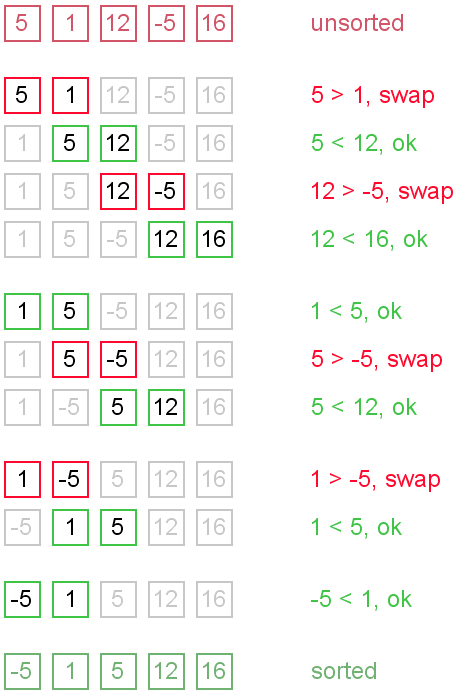
\includegraphics[width= 0.6\textwidth]{figure_man/bubble-sort-1.png}\\
\begin{footnotesize}
\url{http://teerexie.blogspot.com/}
\end{footnotesize}

\end{minipage}

\framebreak

\begin{itemize}
\item The inner loop depends on the outer loop and is executed $i = n - 1$, then $i = n - 2$, ... and finally $i = 1$ times.
\item According to the sum of natural numbers (Carl Friedrich Gauss) the inner loop is executed $\sum_{i = 1}^{n - 1} i = \frac{(n - 1)n}{2} = \frac{n^2 - n}{2}$ times.
\item The operations in the \texttt{if} statement are operations with constant runtime.
\end{itemize}

The total runtime is therefore
$$\frac{n^2 - n}{2} \cdot\order(1) = \order\left(\frac{n^2 - n}{2}\right) = \order(n^2)$$

\framebreak

\textbf{Example 5: } The multiplication of two matrices $\mathbf{A} \in \R^{m \times n}, \mathbf{B} \in \R^{n \times p}$ has a runtime of $\order(mpn)$:

\begin{itemize}
\item $m \cdot p$ scalar products
\item For each scalar product: $n$ multiplications and $n - 1$ additions
\item $\rightarrow$ $m \cdot p \cdot (n + (n - 1))$ operations
\end{itemize}

\begin{center}
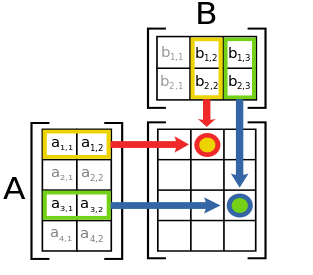
\includegraphics[width= 0.3\textwidth]{figure_man/matrix_multiplication.png}\\
\begin{footnotesize}
\url{https://commons.wikimedia.org/wiki/File:Matrix\_multiplication\_diagram\_2.svg}
\end{footnotesize}
\end{center}


\framebreak
The Coppersmith-Winograd algorithm allows matrix multiplication of two $n\times n$ matrices in $\order(n^{2.373})$. A lower bound for the complexity of the matrix multiplication is $n^2$, since each of the $n^2$ elements of the output matrix must be generated.

\vfill
\begin{footnotesize}
More about \href{https://en.wikipedia.org/wiki/Computational_complexity_of_mathematical_operations}{\color{blue}\underline{Computational complexity of mathematical operations}}
\end{footnotesize}

\framebreak

\begin{verbatim}
multiplyMatrices = function(n) {
  A = matrix(runif(n^2), n, n)
  B = matrix(runif(n^2), n, n)

  return(A %*% B)
}
\end{verbatim}

\vspace{-0.2cm}
\begin{center}
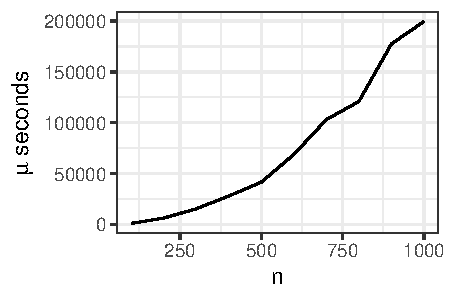
\includegraphics[height = 0.5\textheight, width= 0.6\textwidth]{figure_man/runtime_matmult.pdf}
\end{center}

\framebreak

If possible: Avoid matrix multiplication!
\begin{verbatim}
n = 1000
A = matrix(runif(n), n, n)
B = matrix(runif(n), n, n)
y = c(runif(n))

system.time(A %*% B %*% y)
## user system elapsed 
## 0.72 0.00 0.73

system.time(A %*% (B %*% y))
## user system elapsed 
## 0.00 0.00 0.03
\end{verbatim}

\begin{verbatim}
n = 1000
A = matrix(rnorm(n), n, n) + diag(1, nrow = n)
b = rnorm(n)

# solving Ax = b
system.time(solve(A) %*% b)  # A^{-1} %*% b
## user system elapsed 
## 0.96 0.01 0.05

system.time(solve(A, b)) # direct solution of the LES
## user system elapsed 
## 0.0 0.2 0.0
\end{verbatim}


% \lz
%
% \textbf{Beispiel 5: }
%
% Lösen eines LGS $Ax = b$ mit $\mathbf{A} \in \R^{m \times n}, \mathbf{b} \in \R^{m}$ mit Gauss

\framebreak

\textbf{Example 6:}

In mathematics one is interested in the estimation of error terms for approximations.

Using Taylor's theorem a $m$-times differentiable function $f$ at point $x = x_0$ can be defined as follows:

\begin{footnotesize}
\begin{eqnarray*}
f(x) &=& f(x_0) + \frac{f'(x_0)}{1!}(x - x_0) +  \frac{f'(x_0)}{2!}(x - x_0)^2 + ... +  \frac{f^{(m)}(x_0)}{m!}(x - x_0)^m \\
&+& \order(|x - x_0|^{m + 1}), \quad x\to x_0.
\end{eqnarray*}
\end{footnotesize}

\begin{itemize}
\item The more $x$ approaches $x_0$, the better the Taylor polynomial approximates $f$ at point $x$.
\item The higher the order $m$ of the Taylor polynomial, the better the approximation for $x \to x_0$.
\end{itemize}


\framebreak

For example, consider the exponential function as \textbf{Taylor series}

$$
\exp(x) = \sum_{i=0}^\infty \frac{x^i}{i!}
$$

$\exp(x)$ approximated at the point $x=0$

$$
\exp(x) = 1 + x + \frac{x^2}{2!} + \order(x^3) \text{ for } x \rightarrow 0
$$

In this way, it becomes clear that the error does not become greater than
$M \cdot x^3$ when $x$ approaches $0$.

\framebreak

\textbf{Example 7:}

The complexity of the \textbf{binary search} is visualized by a tree representation.

\begin{center}
  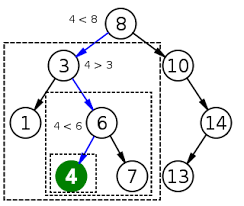
\includegraphics[width=0.3\textwidth]{figure_man/binarysearch.png}
\end{center}

For an array of length $n$, the search tree has a height of $\log_2(n)$. After a maximum of $\log_2(n)$ comparisons, the searched element is found. The complexity of the binary search is $\order(\log n)$.

\framebreak

\textbf{Example 8:}

\footnotesize
The \textbf{Fibonacci sequence} is a series of numbers where each number is the sum of the two preceding ones, starting with 1. The sequence thus begins as:

$1, 1, 2, 3, 5, 8, 13, 21, 34, ...$

\begin{scriptsize}
\begin{verbatim}
fib = function(n) {
  if (n <= 2L)
    return(1L)
  return(fib(n - 2) + fib(n - 1))
}

fib_table = microbenchmark(fib(5), fib(10), fib(20), fib(21), times = 500L)
print(xtable(summary(fib_table), digits = 0), booktabs=TRUE, 
    caption.placement="top", size="\\fontsize{8pt}{9pt}\\selectfont")
\end{verbatim}
\begin{table}[ht]
  \centering
  \begingroup\fontsize{8pt}{9pt}\selectfont
  \begin{tabular}{rlrrrrrrr}
    \toprule
   & expr & min & lq & mean & median & uq & max & neval \\ 
    \midrule
  1 & fib(5) & 2 & 2 & 99 & 3 & 4 & 47817 & 500 \\ 
    2 & fib(10) & 27 & 29 & 32 & 30 & 33 & 88 & 500 \\ 
    3 & fib(20) & 3611 & 3733 & 4164 & 3842 & 4052 & 10118 & 500 \\ 
    4 & fib(21) & 5861 & 6047 & 6926 & 6227 & 6476 & 49636 & 500 \\ 
     \bottomrule
  \end{tabular}
  \endgroup
  \end{table}
\end{scriptsize}

\framebreak

$Fibonacci(n) \in \order(2^n)$ (exponential runtime) \\

\lz

\textbf{Informal proof:}

$$
\texttt{Fibonacci(n)} = \underbrace{\texttt{Fibonacci(n - 1)}}_{T(n-1)} \underbrace{+}_{\order(1)} \underbrace{\texttt{Fibonacci(n - 2)}}_{T(n-2)}
$$

This results in a runtime of $T(n) = T(n-1) + T(n-2) + \order(1)$ for $n >1$.

\lz

The function is executed twice in each step.

\begin{eqnarray*}
  T(n) &=& T(n-1) + T(n-2)  \\
  &=& T(n-2) + T(n-3) + T(n-3) + T(n-4) = \ldots
\end{eqnarray*}

\framebreak

\begin{center}
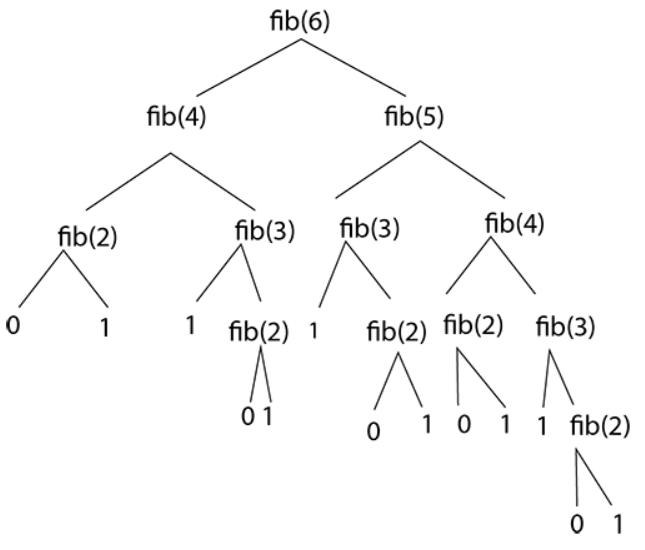
\includegraphics[width=0.5\textwidth]{figure_man/fibonacci.png}
\end{center}

By simply "counting" the nodes of this recursion tree you can determine the exact number of operations. \\
$\to$ Worst case runtime $\order(2^n)$.

\framebreak


\textbf{Variations of Fibonacci(n): Iterative}
\begin{scriptsize}
\begin{verbatim}
fib2 = function(n) {
  a = 0; b = 1
  if (n <= 2)
    return(1)
  for (i in seq_len(n-1L)) {
    tmp = b;  b = a + b; a = tmp
  }
  return(b)
}
\end{verbatim}
\end{scriptsize}
This is $\order(n)$ (if we, incorrectly, assume addition is constant in n).

\framebreak
\begin{scriptsize}
\begin{verbatim}
fib2_table = microbenchmark(fib2(10), fib2(20), fib2(40), fib2(80), 
                            fib2(160), times = 5000L)

print(xtable(summary(fib2_table), digits = 0), booktabs=TRUE, 
    caption.placement="top", size="\\fontsize{8pt}{9pt}\\selectfont")
\end{verbatim}

\begin{table}[ht]
  \centering
  \begingroup\fontsize{8pt}{9pt}\selectfont
  \begin{tabular}{rlrrrrrrr}
    \toprule
   & expr & min & lq & mean & median & uq & max & neval \\ 
    \midrule
  1 & fib2(10) & 1 & 1 & 2 & 1 & 2 & 37 & 5000 \\ 
    2 & fib2(20) & 1 & 2 & 2 & 2 & 2 & 24 & 5000 \\ 
    3 & fib2(40) & 2 & 2 & 4 & 2 & 3 & 6755 & 5000 \\ 
    4 & fib2(80) & 3 & 3 & 4 & 3 & 4 & 26 & 5000 \\ 
    5 & fib2(160) & 5 & 5 & 7 & 6 & 7 & 49 & 5000 \\ 
     \bottomrule
  \end{tabular}
  \endgroup
  \end{table}
\end{scriptsize}
Time measurement becomes imprecise since ``for loops'' are not that slow in \texttt{R} due to JIT compilation. Hence we are using doubles here as a lazy trick to generate large fibonacci numbers. An alternative to generate large integers would be to use the int64 package.\\





\framebreak

\textbf{Variations of Fibonacci(n): In \texttt{C}}

\begin{scriptsize}
\begin{verbatim}
library(inline)
fib3 = cfunction(signature(n="integer"), language="C",
         convention=".Call", body = '
         int nn = INTEGER(n)[0];
         SEXP res;
         PROTECT(res = allocVector(INTSXP, 1));
         INTEGER(res)[0] = 1;
         int a = 0; int b = 1;
         for (int i=0; i<nn-1; i++) {
         int tmp = b;
         b = a + b;
         a = tmp;
         }
         INTEGER(res)[0] = b;
         UNPROTECT(1);
         return res;
         ')
\end{verbatim}
\end{scriptsize}
See how ugly the \texttt{C} interface is?
\framebreak

%\textbf{Variations of fib(n): In C}
\begin{scriptsize}
\begin{verbatim}
fib3_table = microbenchmark(fib3(20L), fib3(40L),times = 5000L)

print(xtable(summary(fib3_table), digits = 0), booktabs=TRUE, 
    caption.placement="top", size="\\fontsize{8pt}{9pt}\\selectfont")
\end{verbatim}

\begin{table}[ht]
  \centering
  \begingroup\fontsize{8pt}{9pt}\selectfont
  \begin{tabular}{rlrrrrrrr}
    \toprule
   & expr & min & lq & mean & median & uq & max & neval \\ 
    \midrule
  1 & fib3(20L) & 300 & 400 & 465 & 400 & 500 & 13900 & 5000 \\ 
    2 & fib3(40L) & 300 & 400 & 479 & 400 & 500 & 21200 & 5000 \\ 
     \bottomrule
  \end{tabular}
  \endgroup
  \end{table}
\end{scriptsize}

This is both $\order(n)$ ... See the difference? Actually, you do not see anything as the function
is so fast, we would need to calculate with bigints to really see the $\order(n)$!

\framebreak

\textbf{Variations of Fibonacci(n): \texttt{C++}-version}
\begin{verbatim}
library(Rcpp)
fib4 = cppFunction('int fibonacci(const int x) {
         if (x <= 2) return(1);
         return (fibonacci(x - 1)) + fibonacci(x - 2);
}
' )
\end{verbatim}

Much nicer \texttt{C++}-Interface with Rcpp.

\framebreak

%\textbf{Variations of fib(n): C++-version}
%\begin{verbatim}
%microbenchmark(fib3(20L), fib4(20L), fib3(40L), fib4(40L))
%\end{verbatim}

%\framebreak


\textbf{Variations of Fibonacci(n): Matrix power-exponentiation}

\begin{footnotesize}
\begin{verbatim}
library(expm)
fib5 = function(n) {
  A = matrix(c(1, 1, 1, 0), 2, 2)
  B = A%^%n
  B[1, 2]
}
\end{verbatim}
\end{footnotesize}

How does \pkg{fib5()} work?

\begin{align*}
  \bm{A} &= \mat{1 & \color{red}{1} \\ 1 & 0} \quad
  \bm{A}^2 = \mat{2 & \color{red}{1} \\ 1 & 1} \quad
  \bm{A}^3 = \mat{3 & \color{red}{2} \\ 2 & 1} \quad
  \bm{A}^4 = \mat{5 & \color{red}{3} \\ 3 & 2} \\
  \bm{A}^5 &= \mat{8 & \color{red}{5} \\ 5 & 3} \quad
  \bm{A}^6 = \mat{13 & \color{red}{8} \\ 8 & 5} \quad
  \bm{A}^7 = \mat{21 & \color{red}{13} \\ 13 & 8} \quad
  \hdots
\end{align*}

\framebreak


\textbf{Matrix power-exponentiation}

What does \verb|A %^% n| do? \\
Computes the n-th power of a matrix corresponding to $n-1$ matrix multiplications
(\verb|A^n| only computes element wise powers).

The algorithm uses $\order(log_2(k))$ matrix multiplications.

\lz
\textbf{Exponentiation by squaring:}

$$
  x^n =
  \begin{cases}
    x(x^2)^{\frac{n-1}{2}} & \text{if n is odd} \\
    (x^2)^{\frac{n}{2}}    & \text{if n is even}
  \end{cases}
$$

\framebreak

\textbf{Exponentiation by squaring}

Implemented as a recursive algorithm:

\begin{scriptsize}
\begin{verbatim}
exp.by.squaring = function(x, n) {
  if(n<0) {
    return(exp.by.squaring(1 / x, -n))
  } else if(n==0){
    return(1)
  } else if(n==1){
    return(x)
  } else if(n%%2 == 0){
    return(exp.by.squaring(x^2, n/2))
  } else {
    return(x * exp.by.squaring(x^2, (n-1)/2))
  }
}
exp.by.squaring(2,5)
## [1] 32
\end{verbatim}
\end{scriptsize}

% Time can not be measured via microbenchmark since it is too fast.
\framebreak

%\textbf{Variations of Fibonacci(n): Matrix power-exponentiation}
%\begin{verbatim}
%microbenchmark(fib5(7), fib5(25L), fib5(49), times = 1000)
%\end{verbatim}


\framebreak


\textbf{Example 9:} The \textbf{Traveling Salesman Problem} (TSP) is the problem of planning a route through all locations in such a way that

\begin{itemize}
\item The entire route is as short as possible,
\item The first location is equal to the last location.
\end{itemize}

\vspace*{-0.2cm}

\begin{center}
  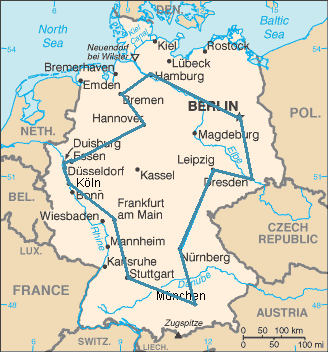
\includegraphics[width=0.3\textwidth]{figure_man/tsp.png}~~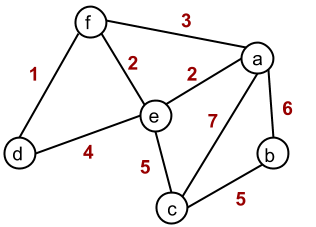
\includegraphics[width=0.4\textwidth]{figure_man/weighted-graph.png}
\end{center}
\vspace*{-0.2cm}

\begin{footnotesize}
Left: Route through places in Germany (\url{https://de.wikipedia.org/wiki/Problem_des_Handlungsreisenden}) \\
Right: Weighted graph (\url{https://www.chegg.com/})
\end{footnotesize}

\framebreak

Exact algorithms with long runtime exist

\begin{itemize}
  \item Brute force search (Calculate lengths of all possible round trips and choose shortest): $\order(n!)$
  \item Dynamic Programming (Held-Karp algorithm): $\order(n^22^n)$
\end{itemize}

and heuristic algorithms with shorter runtime, which do not guarantee an optimal solution, e.g.

\begin{itemize}
  \item Nearest-Neighbor heuristics: $\order(n^2)$
  %\item Minimum-Spanning-Tree-Heuristic: $\order(n^2\log(n))$
\end{itemize}

The TSP problem is \textbf{NP-complete}.

\end{vbframe}


\begin{vbframe}{Complexity classes}

In theoretical computer science, problems are divided into complexity classes. For an input size $n$ a distinction is made between

\begin{itemize}
\item \textbf{P}: Problems solvable in polynomial runtime ($\order(n^k), k\ge 1$)
\item \textbf{NP} (\textbf{N}on-deterministic \textbf{P}olynomial time): Problems from \textbf{P} and problems that cannot be solved in polynomial time;\\ NP problems can only be solved with a non-deterministic turing machine in an acceptable time (hence the name)
\item \textbf{NP-complete}: All problems from NP can be traced back to this problem
\end{itemize}

It has not yet been proven that P $\ne$ NP holds.

\end{vbframe}

\endlecture
\end{document}